%!TEX root = ../dissertation.tex
%\begin{savequote}[75mm]
%Nulla facilisi. In vel sem. Morbi id urna in diam dignissim feugiat. Proin molestie tortor eu velit. Aliquam erat volutpat. Nullam ultrices, diam tempus vulputate egestas, eros pede varius leo.
%\qauthor{Quoteauthor Lastname}
%\end{savequote}

\chapter{Thermalization in an isolated quantum~system}

\section{Statistical mechanics: from  classical to quantum}
Our understanding of statistical mechanics relies on the notion of ergodicity \cite{Penrose1970, Dalessio2016}, which states that during the time evolution a system explores entire phase space allowed by constrains. Time averaging plays an important role in this setup, since the initial conditions of classical non-chaotic system uniquely determine it's state at any particular time during the evolution. Ultimately, time averaging is said to be equal to ensemble averaging \cite{Penrose1970, Dalessio2016}. It's important to note here, that ergodic hypothesis in such setting implies thermalization only in a \textit{weak sense}, where weak refers to the fact that the statement is made only about \textit{time-averaged} values of observables at long times. In order to obtain the thermalization in the \textit{strong sense}, namely, the \textit{instantaneous} values of observables at long times equal to thermodynamic ensemble, one has to consider classical chaotic systems like Fermi-Ulam model \cite{Lichtenberg1992}, the Kapitza pendulum \cite{Broer2004}, and the kicked rotor \cite{Chirikov1979}.

At this point one can ask a question how to translate the classical ideas of thermalization to the quantum language, in particular whether a quantum system can have thermalization in a strong sense? At first glance the it seems illusive, since evolution of a quantum system is governed by the Shr\"odinger equation, which is linear and thus can not provide chaotic dynamics. However recent theoretical breakthroughs \cite{Deutsch1991, Srednicki1994, Rigol2008} have shown that quantum systems also exhibit thermalization. These ideas rely on the conjecture named eigenstate thermalization hypothesis (ETH) \cite{Srednicki1999}, which states that in a chaotic quantum system individual eigenstates are thermal by nature. In order to understand the meaning of this statement, we first need to understand what exactly thermalizes in such systems.

 \begin{figure*}[t]
	\centering
	\includegraphics[scale=2]{figures/ETH_fig1.pdf}
	\caption{{\bf Schematic of thermalization dynamics in closed systems}.  An isolated quantum system at zero temperature can be described by a single pure wavefunction $\vert \Psi \rangle$. Subsystems of the full quantum state appear pure, as long as the entanglement (indicated by grey lines) between subsystems is negligible. If suddenly perturbed, the full system evolves unitarily, developing significant entanglement between all parts of the system. While the full system remains in a pure, and in this sense zero-entropy state, the entropy of entanglement causes the subsystems to equilibrate, and local, thermal mixed states appear to emerge within a globally pure quantum state.  }
	\label{fig:ETH_conceptual}
\end{figure*}

In the early days of quantum mechanics von Neumann noted that, when talking about thermalization, one should focus on local observables rather then wave functions, who carry all global properties of the system (see fig.~\ref{fig:ETH_conceptual}). This approach is very similar to a classical example of isolated container with a gas, where we focus on a small volume inside the container to get a statistical ensemble for the subsystem. From this point of view ETH can be formulated as following: in a quantum chaotic system an expectation value of a local observable is similar between the individual eigenstates and equals to statistical ensemble average. Putting it in more rigorous mathematical terms, ETH states that an expectation value of local observable $O_{nm}$ between eigenstates $\ket{n}$ and $\ket{m}$ is equal to \cite{Srednicki1999}: 
\begin{equation}
O_{nm} = O(\bar{E}) \delta_{nm} + e^{-S(\bar{E})/2} f_O (\bar{E}, \omega) R_{nm},
\end{equation}
where $\bar{E} \equiv (E_n+E_m)/2$, $\omega \equiv E_n-E_m$ and $S(E)$ is thermodynamic entropy at energy $E$. Crucially, $O(E)$ and $f_O(E,ω)$ are smooth functions of their arguments, the value $O(E)$ is identical to the expectation value of the microcanonical ensemble at energy $E$ and $R_{mn}$ is a random real or complex variable with zero mean and unit variance. One important remarks should be made at this point: there are obvious exception form this rule, namely ground state and low lying eigenstates as well as the states on top of the spectrum. Taking this into account, we say that ETH holds for the eigenstates in the middle of the spectrum. 

\section{Quench dynamics of an isolated quantum system}
Unfortunately, there is no known experimental technique to reliably prepare individual exited eigenstates of chaotic Hamiltonians. But since we are interested in dynamics associated with eigenstates in the middle of the spectrum we need to find a way to populate them. Here quantum quenches become handy. Quench is a sudden change in the Hamiltonian parameters, such that the wave function doesn't have time to adjust and, hence, gets reprojected onto the eigenstates of the new Hamiltonian (see fig.\ref{fig:ETH_quench}). Note, that in our experiments we always start in the ground state of the initial Hamiltonian. The energy of this state lies well above the ground state of the final Hamiltonian and the state itself has very small overlap with any of the final eigenstates. Hence, the initial state gets projected onto a large superposition of states primarily in the middle of the spectrum of the final Hamiltonian. 

After the quench the time evolution of the state can formally be written in the basis of final Hamiltonian eigenstates $\ket{n}$ as
\begin{equation}
\ket{\psi(t)}=\sum_n e^{-iE_nt/\hbar}c_n\ket{n},
\end{equation}
where $E_n$ and $c_n$ are corresponding energy and amplitude of the projection. Although this expression looks fairly simple, computing any observable, which is not diagonal in the eigenstate basis, can be very formidable task, since it would involve evaluation of a large number of oscillatory off-diagonal terms. Also, since the energy difference $E_n-E_m$ between different eigenstates can be arbitrary small, those terms would contribute for arbitrary long period of time after the quench. On the other hand, ETH predicts that, for a sufficiently local observable and a states with large entanglement, the contribution of the off-diagonal terms is exponentially small. Hence the expectation value of such observables will be determined by the projection amplitudes $c_n$.

\section{Experimental protocol}
In our experiments we study the emergence of thermalization in a six site chain of interacting Bosons. To initiate the experiment, we isolate a $2 \times 6$ plaquette from a larger low-entropy Mott insulator with unity filling as
shown in figure~\ref{fig:ETH_protocol}. At this point, each system is in a product state of single-atom Fock
states on each of the constituent sites. We then suddenly switch on tunneling along the chains while the tunneling between them is suppressed. Each chain is restricted to the original six sites by introducing a barrier at the ends of the chains to prevent tunneling out of the system. These combined steps realize the setting described in the previous section. Each chain represents an identical but independent copy of a quenched system of six particles on six sites, which evolves in the quenched Hamiltonian for a controllable duration.

In the data that follow, we realize measurements of on-site number statistics and the quantum purity of the state. For measurements of the later, we append to the quench evolution a beam splitter operation that interferes the two
identical copies by freezing dynamics along the chain and allowing for tunneling in a projected double-well potential for a prescribed time~\cite{Islam2015}. In the last step for both measurements, a potential barrier is raised between the two copies and a fullcounting procedure is performed to measure the resulting occupation on each site of each copy.

\section{Local observables in the thermalized pure state}
In order to observe thermalization in our system we first focus on measurements of atom number distributions in various subsystems of the chain. In figure~\ref{fig:ETH_Ensembles}B the number distribution for a single site and half of the chain are shown for two different final values of $U/J = 1.56$ and $U/J =0.38$. The data is averaged in the saturated regime over $5$ times between $10$ and $20~\mathrm{ms}$, and the error bars are the standard deviation in the measured probabilities. We can already make an observation that the standard deviation of measured probabilities is small compared to their value, which indicates that the system is in a quasi-stationary state with small temporal fluctuations around the mean value- a characteristic of a thermal state.

\begin{figure*}[t]
	\centering
	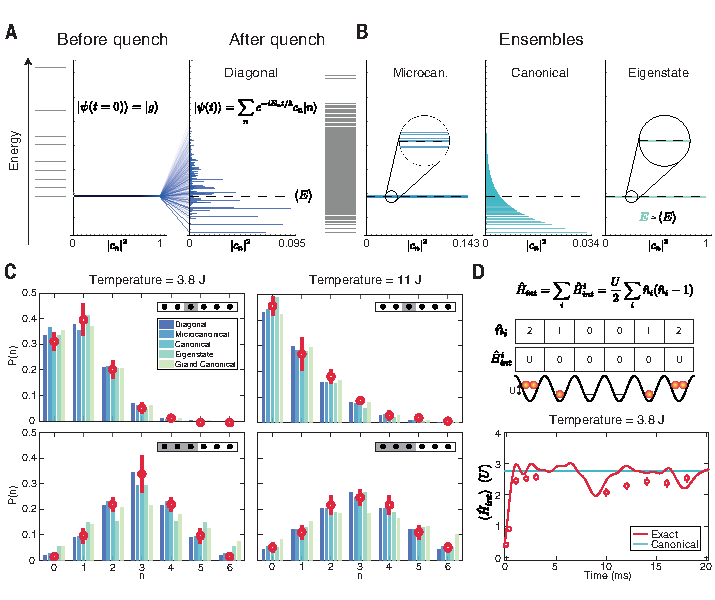
\includegraphics[scale=1]{figures/ETH_fig6.pdf}
	\caption{{\bf Local observables in a globally pure quenched state. } {\bf (A)} Along with the microcanonical ensemble, several other closely related ensembles are compared to the data. {\bf (B)} Thermalization of local observables. For the different temperatures and subsystems shown, the measured number statistics are in excellent agreement with microcanonical and canonical thermal ensembles, verifying the thermal character of the local density matrix. A grand-canonical ensemble reproduces the data very well as long as the subsystem is small compared to the full system. The error bars are the standard deviation of our observation over times between 10 and $20~\mathrm{ms}$.}
	\label{fig:ETH_Ensembles}
\end{figure*}

We compare our measurements to the predictions of thermal ensembles that are illustrated in Figure~\ref{fig:ETH_Ensembles}A, as well as a grand-canonical ensemble truncated to our total atom number~\cite{Appendix}: this ensemble perhaps most closely models how well the many-body state can act as a reservoir for its constituent subsystems. The consistency within the error bars indicates that in this temporal range our observations remain near the thermal predictions despite the presence of temporal fluctuations. For the single site subsystem, the data is in good agreement with all the ensembles considered. Despite the fact that the quenched state is in a large distribution of eigenstates, surprisingly, we find favorable agreement for the case of a single eigenstate ensemble: this illustrates a key principle of ETH, which holds that expectation value of local observables, vary slowly from eigenstate to eigenstate and are therefore relatively insensitive to the width of the distribution of populated states from the quench. We perform the same comparisons to the three-site case in the bottom two panels. Here we also observe agreement with most ensembles, though, interestingly, there is relatively less agreement with the single eigenstate and grand-canonical ensembles, particularly for the lower temperature quench. This variation in agreement may suggest that these ensembles are more sensitive to the relative size of the traced out reservoir compared to the subsystem, which indicates directions of further experiments~\cite{Rigol2012}.


The above measurements were on specific subsystems, but our measurements also allow extraction of the average global interaction energy given by Hamiltonian:
\begin{equation}
\hat{H}_{int}=\frac{U}{2}\sum_i \hat{n}_i(\hat{n}_i-1),
\end{equation}
where $\hat{n}_i$ is the number operator on i-th site and the summation runs over all sites of the chain (see fig.~\ref{fig:ETH_Eint}). Since the interaction Hamiltonian in is diagonal in the Foc basis, we can use our measurements of the final particle configurations to compute the expectation value $\langle \hat{H}_{int} \rangle$. For the $T=3.8J$ data, we show a time scan indicating the initial growth in this quantity, which starts at zero since the initial state is a single particle per site.  These observations, at long times, are in near agreement with the canonical prediction. Interestingly, this measurement is sensitive to the entire six-site system as opposed to some subset of sites, which might suggest that it is global and unlikely to thermalize. Yet, $\langle \hat{H}_{int} \rangle$ undergoes thermalization because it is a sum of local operators, each of which thermalizes and is insensitive to the global purity of the full system.  The observed agreement is consistent with the idea that only a small set of operators, such as the global purity we measure or other specific fine-tuned state projectors, can truly distinguish the pure state we produce from a thermal state.

\section{Thermalization of subsystem density matrix}
We can perform a more rigorous test of single-site thermalization by comparing the measured density matrix of each site with the reduced density matrix of a canonical thermal ensemble $\rho_A^T$ (Figure~\ref{fig:ETH_Rho}B). Our measurements of probabilities to observe a given particle number on a site completely characterize that single-site density matrix, because there are no coherences between different number states due to super-selection rules. With this measured density matrix, we can perform a quantitative comparison to a thermal ensemble using the trace distance ($\frac{1}{2}\mathrm{Tr}(\vert \rho_A^T -  \rho_A \vert)$) and quantum fidelity ($\mathrm{Tr}\left ( \sqrt{\sqrt{\rho_A^T} \rho_A \sqrt{\rho_A^T}}\right )$), both of which quantify the similarity of two mixed quantum states. After a short time, we see a quantum fidelity exceeding $99\%$ and a trace-distance that fluctuates between $0$ and $0.1$, indicating the similarity between the local density matrix of a verified pure state with the local density matrix of a thermal state. The correspondence between the observables of a pure state and thermal state depends on the equivalence of their reduced density matrices within the Hilbert space sampled by the observable. The measurement of Figure~\ref{fig:local}B therefore shows that observables for the single-site Hilbert space should agree with the predictions of thermal ensembles. 